\documentclass[11pt]{article}
\usepackage{../../styles/activity}

\usepackage{xr}
\externaldocument{0-MR}

\lhead{}
%\chead{\textbf{\Large{\hspace{0pt}Beginning Activities for Section~5.1}}\\\hspace{0pt}\emph{Mathematical Reasoning: Writing and Proof}}
\bahead{5.1}
\rhead{}
\lfoot{}
\rfoot{}
\cfoot{\hspace{0pt}\scalebox{0.4}{
\includegraphics{cc-by-nc-sa.eps}}}

\begin{document}

\subsection*{Beginning Activity 1 (Set Operations)}
The examples used in this beginning activity were meant to provide a better understanding of the definitions of set intersection, set union, and set difference. Please note that the correct use of the roster method to describe the sets.
\begin{multicols}{2}
\begin{enumerate}
  \item $A \cup B = \{0, 1, 2, 3, 4, 5, 6, 9 \}$.
  \item $A^c = \{4, 5, 6, 7, 8, 10 \}$.
  \item $B^c = \{0, 1, 7, 8, 9, 10 \}$.
  \item $A \cup B^c = \{0, 1, 2, 3, 7, 8, 9, 10 \}$.
  \item $A^c \cap B^c = \{ 7, 8, 10 \}$.
  \item $A^c \cup B^c = \{0, 1, 4, 5, 6, 7, 8, 9, 10 \}$.
  \item $(A \cap B)^c = \{0, 1, 4, 5, 6, 7, 8, 9, 10 \}$.
\end{enumerate}
\end{multicols}
\hbreak



\subsection*{Beginning Activity 2 (Venn Diagrams for Two Sets)}
Venn diagrams are frequently used in mathematics to explore relationships between sets, and in some situations, to provide counterexamples for false propositions.
\begin{center}
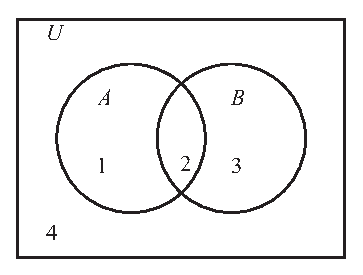
\includegraphics{figps-venn2.eps}
%\caption{Venn Diagram for Two Sets} \label{fig:venn2-prev}
\end{center}

\begin{enumerate}
  \item For the set $A^c$, regions 3 and 4 are shaded.
  \item For the set $B^c$, regions 1 and 4 are shaded.
  \item For the set $A^c \cup B$, regions 2, 3, and 4 are shaded.
  \item For the set $A^c \cup B^c$, regions 1, 3, and 4 are shaded.
  \item For the set $(A \cap B)^c$, regions 1, 3, and 4 are shaded.
  \item For the set $(A \cup B) - (A \cap B)$, regions 1, and 3 are shaded.
\end{enumerate}
\hbreak

\end{document}

